\chapter{浮游动物图像分类基础}

\section{机器学习分类技术}

利用机器学习方法对浮游动物图像进行分类的主要模块是图像预处理、特征提取、分类,主要步骤为:

(1)将浮游动物图像样本分为训练样本和测试样本两类,并建立实验所需的训练样本和测试样本数据;
(2)分别对训练样本和测试样本进行预处理;
(3)对训练样本进行特征提取,从中选择合适的特征信息构成特征向量;
(4)设计分类算法,通过支持向量机、随机森林、神经网络等方法设计分类器;
(5)将训练样本图像的特征输入到分类器,训练出分类模型;
(6)提取测试样本特征,并输入到分类模型中,输出测试样本的分类结果。具体见图~\ref{fig: ClassificationFlowchart}。

\begin{figure}[h] %插图
\centering
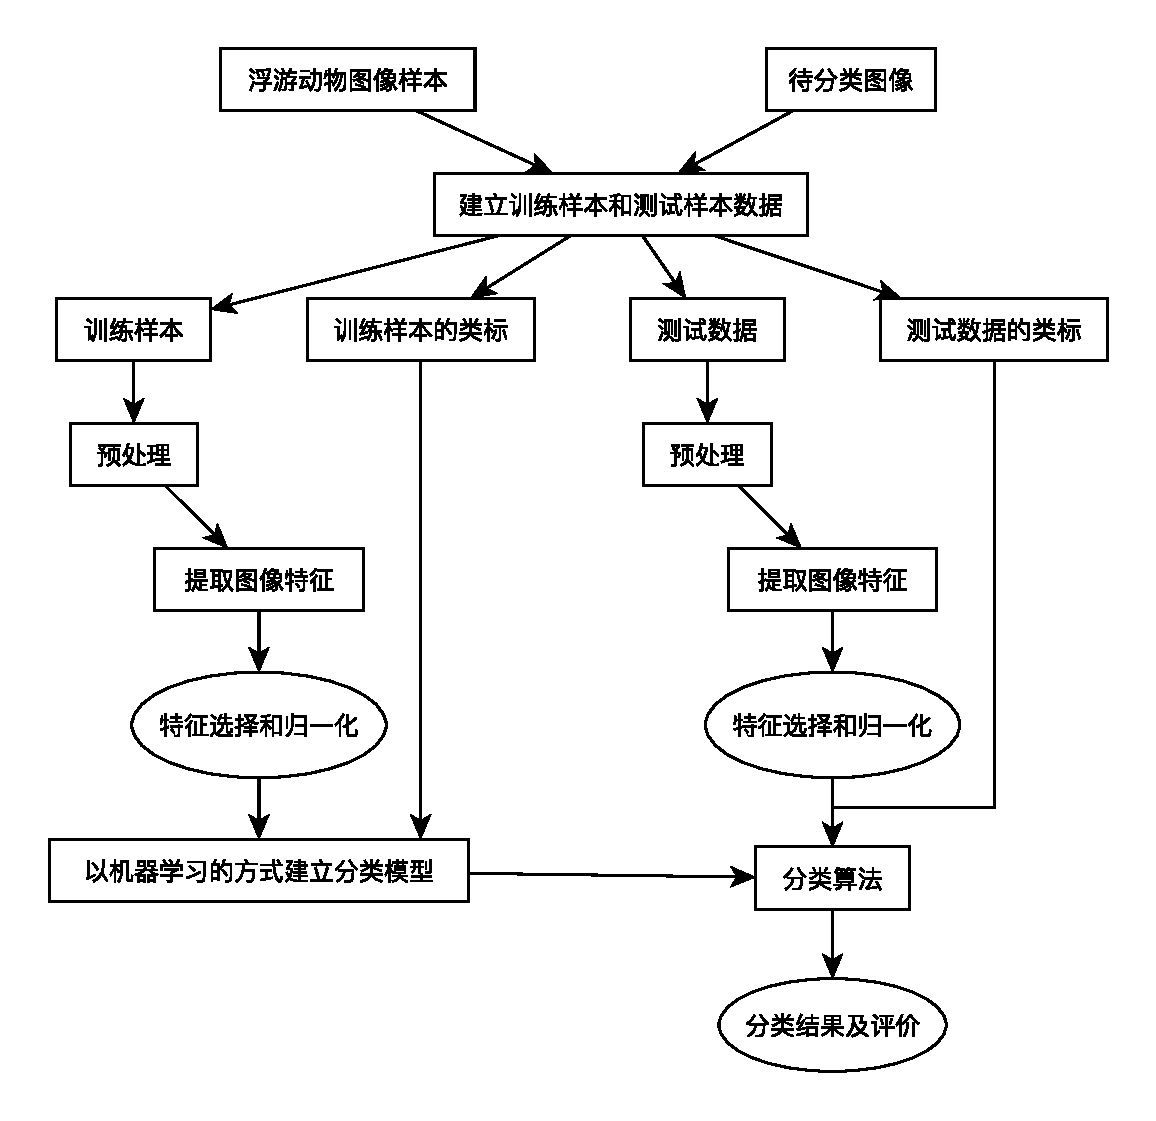
\includegraphics[width=0.6\textwidth]{ClassificationFlowchart.eps}
\caption{利用机器学习方法实现浮游动物图像分类的基本流程}
\label{fig: ClassificationFlowchart}
\end{figure}

\section{数据集}
\label{2.1}

自1949年起,加利福尼亚海洋渔业研究合作组织(California Cooperative Oceanic Fishery Investigation, CalCOFI)就开始对包括浮游生物在内的海洋生物进行采样~\cite{bograd2003calcofi},根据标准邦戈网络协议采集海洋中的浮游生物样本,然后立即保存起来。部分被保存的CalCOFI样本被连接到加利福尼亚对当前生态系统进行长期生态研究的网站上,并用ZooScan进行了扫描~\cite{gorsky2010digital}。得到的灰度图像质量较好,在对比度、噪声等方面都得到了精确控制。整个数据集包含的种类如表~\ref{表1}所示,其中每种类别图像所占比例见图~\ref{fig: ratio},以下对该数据集中的每一类别分别进行了详细说明和描述。

\begin{table}[htbp]
\centering
\caption{浮游动物数据集包含种类}
\begin{tabular}{|r|l|}
\hline
Appendicularia & 尾海鞘纲 \\
Bubble & 气泡 \\ 
Chaetognatha & 毛颚动物门 \\
Cladocera Penilia & 尖头溞属 \\
Copepoda & 桡脚类 \\
Decapoda & 十足目 \\
Doliolida & 海樽目 \\
Egg & 卵 \\
Fiber & 纤维 \\
Gelatinous & 明胶 \\
Multiple & 多个生物 \\
Pteropoda & 翼足目 \\
Nonbio & 非生物 \\
\hline
\end{tabular}
\label{表1}
\end{table}

\begin{figure}[!ht]
\centering
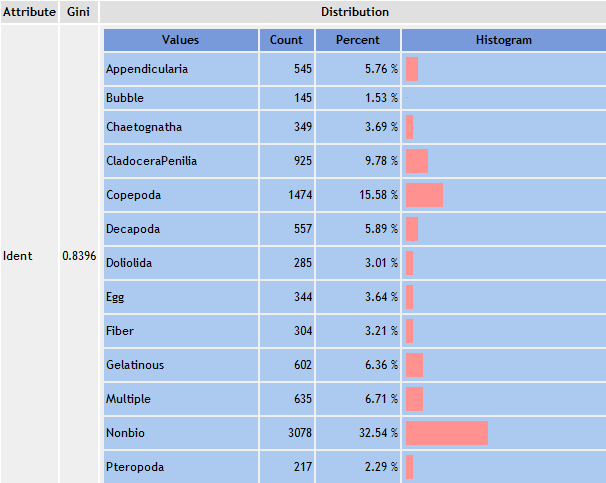
\includegraphics[width=0.6\textwidth]{每个类别所占比例.png}
\caption{数据集中每种类别的数目及所占比例}
\label{fig: ratio}
\end{figure} 

\begin{description}
    \item[Appendicularia(尾海鞘纲)] 属于脊索动物门,体型像蝌蚪,身体分为躯干和尾两部分。躯干较大且灰度较深,呈不太规则的椭圆形。尾部比躯干要长,长度大多小于5mm。尾部大致呈现两种形状:一种细长弯曲,另一种较粗(粗细甚至于头部差不多),呈现柳叶状。尾部的灰度相比于躯干较浅,轮廓不太清晰。

    \item[Bubble(气泡)] 非生物,圆形。气泡四周灰度深,中间灰度很浅,呈亮白色。

    \item[Chaetognatha(毛颚动物门)] 身体修长,可以明显看出身体分为头、躯干和尾3部分。头部略膨大,躯干与头连接处稍微缢缩为颈部,躯干较粗,轮廓清晰。尾部慢慢变窄,末端尖细。头部两侧各着生一列4~13根镰刀状、几丁质的颚毛。大小:最大成年成年个体长105mm,该类成年个体的长度一般都大于5mm。

    \item[Cladocera Penilia(Penilia,尖头溞属)] 属于节肢动物门,鳃足纲,枝角目,俗称水跳蚤。身体短小,有两条长长的触角。该类浮游动物身体中轴线的地方灰度较深(感觉类似人体的脊柱),这个颜色较深的中轴线上还有一条条纹理线连向边缘(就像人体脊柱上连着的骨骼)。由于运动,扫描得到的图像中浮游动物的中轴线并不是都在其身体中间。大小约为1mm左右。
    
    \item[Copepoda(桡脚类)] 属于节肢动物门,颚足纲,桡足类属于其下的一个亚纲。体形像泪珠,有大的触角。分为前体部和后体部,前体部较为宽大,后体部较为短小。前体部前体部由头和胸部组成,头部有两对触角,胸部有鄂足、五对胸足。后体部无附肢,由3—5节组成。最末的腹节称尾节,末端具1对尾叉,尾叉的末端有5根不等长的刚毛,常呈羽状。    
    
    \item[Decapoda(十足目)] 属于节肢动物门,软甲纲。又分为两类:Lucifer hanseni和Crab larvae。体躯延长呈虾形(腹部发达)或缩短扁圆呈蟹形(腹部化)。

    \item[Doliolida(海樽目)] 属于脊索动物门,樽海鞘纲。体型一般呈桶状,体壁最外是被囊层,其内层是外套膜。被囊层下有8~9条肌带环绕着体躯。由于该类浮游动物比较透明,因此在图像中灰度较浅,并且其桶状轮廓也不完整了,但最明显的是能看到大概7、8条环状的肌肉带,有的图像中还能看到内部器官。

    \item[Egg] 很多种类生物的卵。形状大致都呈圆形。有的卵整体灰度都很深;有的卵中间有一块灰度较深的区域,四周灰度较浅(结构像细胞)。由于是不同动物的卵,因此其灰度特征差异较大。

    \item[Fiber(纤维)] 非生物。弯曲的线状,有的纤维有分叉和交叉。该类图像中噪声较多,纤维的边缘也不是很规则。

    \item[Gelatinous(明胶)] 该类包括很多不同种类的胶状生物,它们体内都含有很高的水分。包括Aglaura(属于刺胞动物门)、Medusa(水母,属于刺胞动物门,水螅纲)、Siphonophora(管水母,属于刺胞动物门,水螅纲,管水母目)、Radiolaria(放射虫,属于原声动物门,辐足纲)和Salps(樽海鞘,属于脊索动物门Chordata,樽海鞘纲Thaliacea,纽鳃樽目Salpida)。其中水母大部分都有三个主要部位:圆伞状或是钟状(寺院里面敲得那种钟)的身体、触器和口腕。由于该类呈胶状,因此该类物体灰度整体较浅,边缘也不是十分清晰。大部分是水母,有小部分的樽海鞘(与海樽目形态很相似),小部分的放射虫。
        \item 其中水母也包括很多类,形态大致呈现以下几种:
            \begin{itemize}
            \item 一些水母身体呈现类似钟状(这里呈现钟状有长有短,有粗有细,还有的会发生一点弯曲),灰度较浅,内部有一块颜色较深的椭圆形区域。
            \item 一些水母也呈钟状,但内部没有颜色较深的椭圆形区域,整个身体灰度均匀。
            \item 还有的个头稍微偏小,形状有的类似圆形、像半个胶囊(应该是由于拍摄原因,有的拍到顶部,有的拍到侧面),体内有颜色较深的一个大点和几个小点。(可能是灯塔水母)
            \end{itemize}
        \item 放射虫:形状近似圆形(但由于整体灰度较浅,形状保存是完整),中间有一块灰度较深的区域,四周灰度较浅,可以看到淡淡的细纹从中心连接到边界。
        
    \item[Multiple(多个生物)] 由于浮游动物的重叠,导致分割过程中多个浮游动物被分割到一张图像上。
    
    \item[Pteropoda(翼足目)] 属于软体动物门,腹足纲。该类浮游动物灰度较深,形状总体都呈现一头宽一头窄。形状总体呈现三类:有的呈现象牙状,有点弯曲;有的较粗短,像一顶尖的小帽子;有的呈现细长的三角形状。
    
     \item[Nonbio] 非生物的集合。
\end{description}

\section{评价方法}

\subsection{混淆矩阵简介}
\label{CM}

在机器学习中,混淆矩阵(CM)是一种比较简单的对分类模型的性能进行评价的评估准则,主要用于比较分类结果和实际测得值。混淆矩阵是一个$n$行$n$列的矩阵,$n$代表类别的数量。矩阵的每一列代表预测的每一类的数量,每一行代表实际的每一类的数量。对角线上表示分类正确的每一类的数量。例如:有180个样本数据,这些数据实际分为3类,每类60个,分类结束后得到的混淆矩阵如表~\ref{ConfusionMatrixExample}所示。第一行说明类1的60个样本有53个样本分类正确,5个错分为类2,2个错分为类3。第一列说明类1有53个样本分类正确,类2的2个样本被错分为类1,类3没有样本被错分为类1。对角线上的数据表示,类1、2、3分别有53、55、59个样本被分类正确。
    
\begin{table}[ht]
\centering
\caption{混淆矩阵例子}
\begin{tabular}[c]{|c|c|c|c|}
\hline
 & 类1 & 类2 & 类3\\
 \hline
类1 & 53 & 5 & 2 \\
\hline
类2 & 2 & 55 & 3\\ 
\hline
类3 & 0 & 1 & 59\\ 
\hline
\end{tabular}
\label{ConfusionMatrixExample}
\end{table}

根据混淆矩阵可以导出以下几个参数:
\begin{itemize}
    \item true positives (TP):正样本被识别出的数量
    \item true negatives (TN):负样本被识别出的数量
    \item false positives (FP):负样本被错误分为正样本的数量
    \item false negatives (FN):正样本被错误分为负样本的数量 
    \item Accuracy:准确率,针对分类器的整个预测情况。
        \begin{displaymath}
            Accuracy=\frac{TP+TN}{TP+TN+FP+FN}
        \end{displaymath}
    \item {Error rate:误分类率,针对分类器的整体预测情况。}
        \begin{displaymath}
            Error rate=\frac{FP+FN}{TP+TN+FP+FN}
        \end{displaymath}
    \item {The true positive rate (TPR) :召回率,正样本被识别出的概率。}(文中和PkID中使用的评价参数)
        \begin{displaymath}
            TPR=\frac{TP}{TP+FN}
        \end{displaymath}
     \item The false positive rate (FPR):虚警率,负样本被错误分为正样本的概率。
        \begin{displaymath}
            FPR=\frac{FP}{FP+TN}
        \end{displaymath}
    \item The true negative rate (TNR):负样本被识别出的概率
        \begin{displaymath}
            TNR=\frac{TN}{FP+TN}
        \end{displaymath}

    \item The false negative rate (FNR) :漏警率,正样本被错误分为负样本的概率。
        \begin{displaymath}
            FNR=\frac{FN}{FN+TP}
        \end{displaymath}
    \item {False discovery rate (FDR):1-precision。}(文中和 PkID 中使用的评价参数)
        \begin{displaymath}
            FDR=\frac{FP}{FP+TP}
        \end{displaymath}
    \item Positive predictive value (PPV)
        \begin{displaymath}
            PPV=\frac{TP}{TP+FP}
        \end{displaymath}
    \item Negative predictive value (NPV)
        \begin{displaymath}
            NPV=\frac{TN}{TN+FN}
        \end{displaymath}
    
\end{itemize}

\subsection{混淆矩阵分类}

根据训练集和测试集的不同选取方式,混淆矩阵可以通过以下两种方式得到:
\begin{enumerate}
\item Re-substitution混淆矩阵       
当采用的测试集和训练集为同一个数据集时,得到的混淆矩阵叫做Re-substitution混淆矩阵。在这个过程中,用产生的分类器对测试集进分类时,得到的分类结果错误较少甚至可能没有错误,在进行评价时就会低估分类器的错误率。
\item 交叉验证混淆矩阵
采用交叉验证(交叉验证介绍见~\ref{Cross Validation})的方法得到的混淆矩阵就叫做交叉验证混淆矩阵。并且这里采用的训练集和测试集之间在样本上是没有重合的。首先将一个数据集分成$K$个相等的子集,用其中$K-1$个子集来训练产生分类器,用剩下的1个子集来进行测试,重复进行$K$次来构建混淆矩阵。
\end{enumerate}

\subsection{交叉验证}
\label{Cross Validation}
交叉验证是用来评价分类器的分类性能的一种方法,其基本步骤是是对原始图像集进行分组,然后选择没有交叉的两部分,一部分用作训练,一部分用作测试,用得到的混淆矩阵来评价分类器的性能好坏。

在机器学习的常见算法中,首要的步骤通常是将数据集分为训练集和测试集两个子集,其中训练集用来建立模型,而测试集则用来评价该模型对未知样本进行预测时的准确度,即泛化能力。如何将完整的数据集分为训练集跟测试集,必须遵守以下几条要点:
\begin{enumerate}
    \item 在训练分类器阶段用到的是训练集,不能使用测试集,训练完成后再在测试集上测试分类效果,将两者在分类器建立前后做到严格分离。
    \item 一般来说,训练集中图像数量要多于测试集,以保证训练出的分类器有效。
    \item 对于训练集和测试集,都必须做到对原始数据中每一类都均匀采样,不能过分偏向其中某几类,这样会导致训练出的分类器没有将所有类别的特点都考虑进去。
\end{enumerate}

常见的交叉验证形式有Holdout验证、$K$折交叉验证和留一验证三种,其中用的比较多是$K$折交叉验证。首先将原始的整个图像集平均分成$K$份,一般是随机挑选分配。每一次训练分别将其中一份作为训练集,另外的$K-1$份作为测试集,得到一个混淆矩阵,由于有$K$份,所以会进行$K$次训练和测试,得到$K$个混淆矩阵,将这$K$个混淆矩阵累加起来,就能得到$K$折交叉验证的混淆矩阵。$K$的取值通常大于等于2。在将图像集分成子集时由于是随机分配的,带有一定的随机性,所以在实际应用中,为了避免随机性对分类器效果的影响,我们通常会随机分配$n$次,将每一次得到的$K$折交叉验证的混淆矩阵进行叠加,得到最终的混淆矩阵。

本文中对分类结果采用$K$折交叉验证方式得到的混淆矩阵进行评价,其中$K$取值为2,$n$取值为5,对混淆矩阵计算Recall和1-Precision值,得到每一类的分类准确率和错误率,再对所有类别求平均,得到对整个数据集进行分类的分类准确率和错误率。

\section{ZooScan系统介绍}

利用机器学习方法进行浮游动物图像分类的方法有很多,目前取得最好的分类效果的是法国国家科学研究院研制的ZooScan系统~\cite{gorsky2010digital},受到该系统的启发,我们对其中的浮游动物图像特征提取和分类器设计两个关键环节进行了更深入的研究,从而对其进行了有效的改进,使分类准确率进一步提高。下面具体介绍ZooScan系统的主要组成部分。

\subsection{简介}

ZooScan Integrated System是由法国国家科学研究院Villefranche海洋实验室的Gorsky等人发明、Hydroptic公司生产的浮游动物样品图像扫描和处理系统,能够快速实现对液体中的浮游动物样品的扫描、计数、种类鉴定和生物量的测定,目前在国内和国外都影响很广。

ZooScan系统是由ZooScan、ZooProcess和Plankton Identifier (PkID)三个部分组成的,其中前者是系统的硬件部分,用来对液体中的浮游动物样品进行扫描,得到高分辨率的数字图像。后两者是软件部分,先对扫描得到的图像进行一些标准化处理,对个体的一些形态、几何、灰度等参数进行提取,然后利用一些基本的机器学习算法对特征进行训练,得到分类器,最终实现对浮游动物图像的分类识别。

\begin{figure}[!ht] %插图
\centering
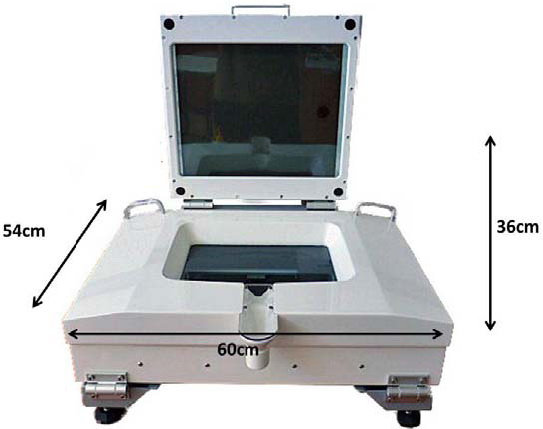
\includegraphics[width=0.4\textwidth]{ZooScan.jpg}
\caption{ZooScan主扫描区}
\label{fig: ZooScan}
\end{figure}

\subsection{硬件部分}

ZooScan系统的扫描设备分为了上下两个部分(图~\ref{fig: ZooScan}),为了能够扫描带液体的样本,对设备的防水性有较高的要求,ZooScan扫描系统在这方面作了很好地处理,其内部隔绝水的性能相当好。扫描设备的上面部分提供了两种功能,一是照明,二是进行光密度的检测。下面部分是扫描区域,即液体样本的放置地方。由于扫描时光是从空气进去水中,再从水中进入玻璃,要分两次完成在两种不同介质之间的穿透,因而在成像效果上会相应差一些,表现为图像分辨率的降低。针对浮游动物样本的不同尺寸,ZooScan系统提供了$1200dpi$和$2400dpi$两种分辨率以及$11cm\times24cm$和$15\times24cm$两种大小的扫描框以供选用。

\begin{figure}[!ht] %插图
\centering
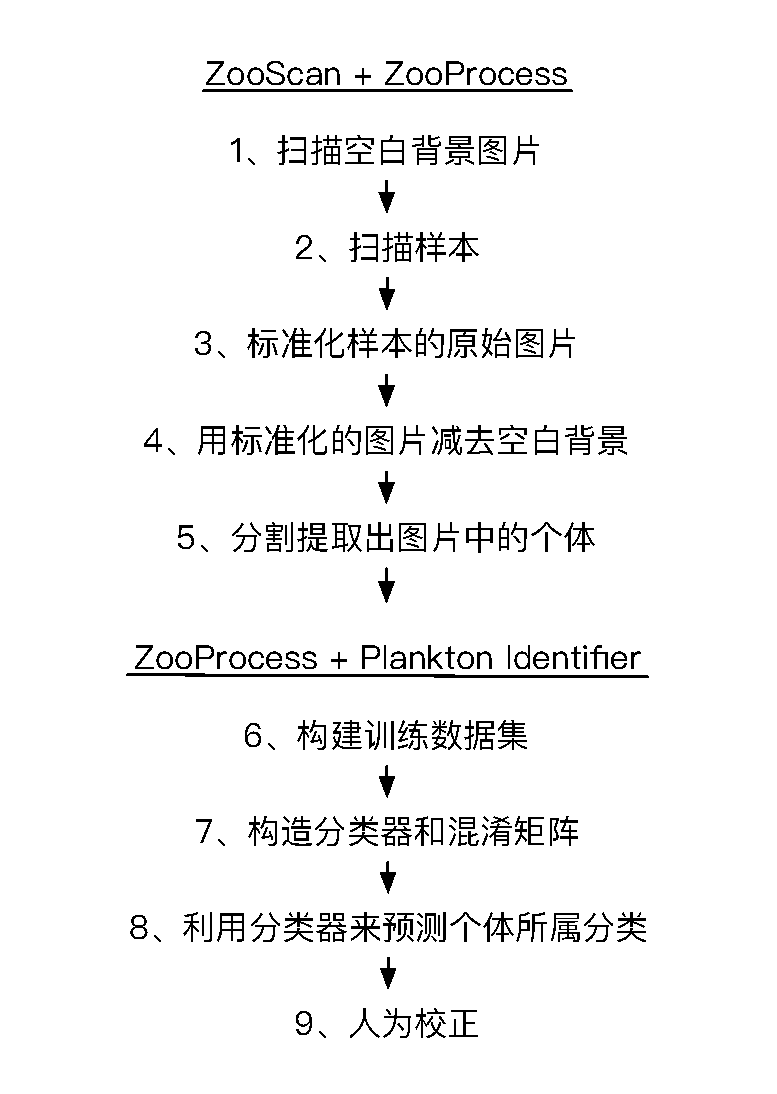
\includegraphics[width=0.4\textwidth]{ZooScanFlowchart.eps}
\caption{利用机器学习方法实现浮游动物图像分类的基本流程}
\label{fig: ZooScanFlowchart}
\end{figure}

\subsection{软件部分}
\label{2.3.3}

利用ZooScan系统对浮游动物进行扫描和分析的基本步骤如图~\ref{fig: ZooScanFlowchart}所示。最初的步骤是使用ZooProcess软件完成:(i)扫描空白背景图片,(ii)扫描样品以获得高质量的原始图片和元数据信息,(iii)标准化原始图片,(iv)去掉扫描框的边缘,以空白背景校正图片,(v)分割提取并测量图片中的个体。随后的分析步骤是利用ZooProcess结合PkID完成:(vi)构建训练数据集,(vii)构造分类器和混淆矩阵,(ix)利用分类器来预测个体所属分类,(x)人为校正。下面会详细说明这些步骤。

\begin{enumerate}
\item 扫描空白背景图片

在扫描空白背景图片前需要打开ZooProcess软件创建一个新的项目,设置扫描参数,有$1200dpi$和$2400dpi$两种分辨率可供选择。然后输入样本的元数据信息。

背景图像是一张空白图像,在与样品相同环境下(自来水或是过滤海水),先扫描背景再扫描样品。并且最好是在每个扫描任务开始时,都扫描一次背景图像。首先用清水清洁和冲ZooScan 托盘和表面玻璃,时不时地检查并清除在玻璃和扫描框上的污点。然后倒一些清水(保持在室温)没过托盘,它可以防止扫描框刮擦托盘。再放置扫描框($15cm \times 24cm$),这取决于之前 ZooProcess 中的“创建项目”中的选项。在预扫描和实际扫描之间,等待 30 秒。

\item 扫描样品以获得高质量的原始图片和元数据信息

首先需要准备好样品,存储几升清水,保持在室温,用来为 ZooScan 注水。然后用筛子(网格间隙为$100\mu m$)过滤掉防腐剂和海水中物质。样品通过间隙为$1mm$和$200\mu m$的两种网格,将浮游生物分成不同体型的两部分。分别将分开后的样品,添加标签$d1$和$d2$,用于扫描后的数据处理过程中。使上述两个分开后的样品中,保持只有 $1000 − 1500$ 个浮游生物。

在扫描托盘中加入量水,放置扫描框($15cm \times 24cm$),调整扫描框放置的位置(位置在扫描托盘中有标注)。倒入样品,加入清水,直到没过扫描框的台阶。将个体较大的浮游生物放在扫描框的中心,用木棒分离粘连浮游生物,避免浮游生物贴靠扫描框边缘。对于漂浮在水面的浮游生物,轻轻用木棒将浮游生物压入水中。如果存在无法没入水中的浮游动物,且数量不多,则将它们移出。检查托盘是否有气泡,顶盖玻璃的表面是否冷凝。加载 ZooProcess,选择项目,点击扫描样品,选择两部分样品中的一个样品($d1$和$d2$)。扫描完成后,输入相关元数据,用于将来的使用和比较。

\item 标准化原始图片

对扫描图片进行标准化可以允许使用不同参数得到的扫描图片之间进行转化和运算。对扫描图片和背景图片都要进行标准化,然后再进行相减操作。其中灰度和尺寸大小是浮游动物自动识别过程的两个最重要的变量,16位的原始图片可以通过计算黑点(Black point, Bp)和白点(White point, Wp)转化为8位图片。
\begin{align}
Wp = Mg \cdot 1.15\\
Bp = \frac{Mg}{1.15 \cdot log(OD)}
\end{align}
其中,Mg(Median grey level)表示图片的平均灰度值,OD表示光密度值。

\item 去掉扫描框的边缘,以空白背景校正图片

对标准化后的原始图片和空白图片进行相减。

\item 分割提取并测量图片中的个体

默认的分割灰度值为243,等周长直径(Equivalent Circular Diameter, ECD)大于$0.3mm$的个体会被检测出来并进行下一步处理。

\item 相关参数提取

ZooProcess中对个体提取的参数一共有67个:Area, Mean, StdDev, Mode, Min, Max, X, Y, XM, YM, Perim., BX, BY, Width, Height, Major, Minor, Angle, Circ., Feret, IntDen, Median, Skew, Kurt, \%Area, XStart, YStart, Area\_exc, Fractal, Skelarea, Slope, Histcum1, Histcum2, Histcum3, XMg5, YMg5, Compentropy, Compmean, Compslope, CompM1, CompM2, CompM3, Symetrieh, Symetriev,Tag, ESD, Elongation, Range, MeanPos, CentroidsD, CV, SR, PerimAreaexc, FeretAreaexc, PerimFeret, PerimMaj, Circexc, CDexc, Nb1, Nb2, Nb3,  Symetriehc, Symetrievc, Convperim, Convarea, Fcons, ThickR。大致可以分为位置特征、尺寸特征、灰度特征、形状特征、生物统计特征、自定义特征六大类。

\begin{enumerate}
\item 位置特征
\begin{description}
\item[BX、BY] 能够包围物体,且平行于图像两条边的最小外界矩形的左上角顶点的X坐标和Y坐标。
\item[Height、Width] 能够包围物体,且平行于图像两条边的最小外界矩形的高和宽。
\item[XStart、YStart] 图像最左上角像素点的X坐标和Y坐标。
\item[XM、YM] 物体灰度重心的X坐标和Y坐标。
\item[XMg5、YMg5] gamma值为51时的物体灰度重心的X坐标和Y坐标(gamma值表示图像输出值与输入值关系的斜率)。
\item[X、Y] 物体重心点的X坐标和Y坐标。
\item[Angle] 浮游动物主轴与图片x轴形成的夹角,在图片切割后旋转图片测量相关参数使用。
\end{description}
这类特征反映的是浮游动物在图像中的位置信息,浮游动物特征与位置信息无关,因此它们不适合作为特征直接用于分类(会降低分类的准确率),而是用来计算其他特征(尺寸特征、灰度特征和形状特征)。

\item 尺寸特征

\begin{description}
\item[Area] 包含物体的最小矩形面积 。
\item[Perim] 周长,物体最外层边缘的长度。
\item[Major] 物体的最佳拟合椭圆的长轴。%物体内切椭圆的长轴
\item[Minor] 物体的最佳拟合椭圆的短轴。%物体内切椭圆的短轴
\item[Feret] Maximum feret diameter(最大费雷特径), 沿物体边缘任意两个点的最长距离。
\item[Area\_exc] 去掉物体空洞后的表面积,空洞是指灰度值与背景相同的部分。
\item[\%area] 物体表面积中空洞所占的百分比,即背景所占的比例。
\end{description}

这类特征表示了图像中目标的大小尺寸。它的根据是同类浮游动物的表面积、周长等尺寸特征应该是大致相同的。但是这些特征还存在着问题:1、同类浮游动物在不同时期(如幼年和成年)的个体大小尺寸是不同的。2、拍摄照片的方位不同(比如正面和侧面),得到的尺寸特征也是不同的。

\item 灰度特征

\begin{description}
    \item[Min、Max] 物体内部所有像素点的最小灰度值和最大灰度值(0 = black,255 = white)。
    \item[IntDen (Integrated density)] 总密度,物体内像素点的灰度值的总和($IntDen = Area * Mean$)。
    \item[Slope] 归一化的灰度累计直方图的斜率。
    \item[Histcum1] 灰度累计直方图的值为25\%时所对应的灰度值。
    \item[Histcum2] 灰度累计直方图的值为50\%时所对应的灰度值。
    \item[Histcum3] 灰度累计直方图的值为75\%时所对应的灰度值。
    \item[CentroidsD] $\sqrt{(XM-X)^{2}+(YM-Y)^{2}}$ 目标物体重心和灰度重心之间的距离。
    \item[Fcons] 灰度对比度。
    \item[Nb1] 图像在用阈值Histcum1二值化后剩余对象的数量。
    \item[Nb2] 图像在用阈值Histcum2二值化后剩余对象的数量。
    \item[Nb3] 图像在用阈值Histcum3二值化后剩余对象的数量。
    \item[ThickR] 物体最大厚度和平均厚度(不包括最大厚度)的比值。
\end{description}

利用灰度特征进行浮游动物图像分类的依据是同类浮游动物的灰度特征(灰度的范围和整体灰度变换趋势)应该是相似的。但观察图像发现并不是所有同类浮游动物的灰度都是相似的,例如Gelatinous类中有的个体灰度跨度较小,整体灰度都较浅,而有的个体灰度跨度较大。同时由于拍摄时光线的原因,也会造成同类浮游动物中个体灰度的深浅不一。

\item 形状特征

\begin{description}
    \item[Fractal] 物体边界的分形维数,表明物体边界的不规则程度。
    \item[Skelarea] 骨架像素的表面积(在二值图像中,不断地从物体边缘处减去像素点直到仅剩一个像素的宽度,最后所得图形的像素点数)。
    \item[Symetrieh] 关于水平轴的对称性。
    \item[Symetriev] 关于竖直轴的对称性。
    \item[Symetriehc] 图像在用阈值Histcum1二值化后物体的水平对称性。
    \item[Symetrievc] 图像在用阈值Histcum1二值化后物体的垂直对称性。
    \item[Circ] $Circularity = (4 * Pi * Area) / Perim^2$ 圆形度,表征物体接近圆的程度,值等于1时,说明物体为正圆形,值越接近0,物体体形越长。
    \item[ESD] $2 \times \sqrt{\cfrac{Area}{\pi}}$ 相应球形直径(也称为等效球直径),是指一不规则外形物体,其体积相同球体的直径。
    \item[Elongation] $\cfrac{Major}{Minor}$ 延伸率,最佳拟合椭圆的长轴和短轴之比。
    \item[Circexc] $\cfrac{4 \times \pi Area\_exc}{Perim^{2}}$ 去掉目标内部空洞的圆形度。
    \item[Convperim] 包围物体凸包的周长。
    \item[Convarea] 包围物体凸包的面积。
\end{description}

这类特征描述的是浮游动物的形状特征,依据是不同种类浮游动物之间形状不同。但在本文所采用的数据集中存在的问题是有不同种类的浮游动物形状相似,例如Appendicularia和Chaetognatha,Bubble和Egg,也有同种浮游动物形状不同,例如Decapoda、Gelatinous。

\item 生物统计特征

\begin{description}
    \item[Mean] 物体内的平均灰度值,物体中所有像素点的灰度值的总和除以总的像素个数。
    \item[Range] $Max-Min$ 极差,灰度的范围。    
    \item[CV] $100 \times \cfrac{StdDev}{Mean}$ 变异系数(也称离散系数或相对偏差),是灰度标准偏差与平均值之比,用百分数表示。
    \item[SR] $100 \times \cfrac{StdDev}{Max-Min}$ 灰度标准差比上极差。
    \item[Skew] 灰度直方图的偏度,衡量灰度分布的不对称性。正态分布的偏度为0,概率密度函数两侧的尾部长度互相对称。偏度为负表示概率密度函数左侧的尾部相对于右侧要长,大部分的值位于平均值的右侧。偏度为正表示概率密度函数右侧的尾部比左侧的长,即处于平均值左侧的值要比右侧多。
    \item[Kurt] 峰度,描述灰度直方图的陡缓程度。 
    \item[Mean\_exc] 物体内部去掉空洞后的平均灰度值($Mean\_exc = IntDen / Area\_exc$)。
    \item[Median] 物体内像素的灰度值的中值。
    \item[StdDev] 物体内像素的灰度值的标准差。
    \item[Mode] 表示灰度的众数。
\end{description}

\item 自定义特征
\begin{description}
    \item[MeanPos] $\cfrac{Mean-Max}{Max-Min}$
    \item[PerimAreaexc] $\cfrac{Perim}{\sqrt{Area\_exc}}$ 
    \item[FeretAreaexc] $\cfrac{Feret}{\sqrt{Area\_exc}}$
    \item[PerimFeret] $\cfrac{Perim}{Feret}$
    \item[PerimMaj] $\cfrac{Perim}{Major}$
    \item[CDexc] $\cfrac{\sqrt{(XM-X)^{2}+(YM-Y)^{2}}}{{\sqrt{Area\_exc}}}$ 
    \item[ESD] $2 \times \sqrt{\cfrac{Area}{\pi}}$
    \item[Elongation] $\cfrac{Major}{Minor}$
    \item[Range] $Max-Min$
    \item[CentrodisD] $\sqrt{(XM-X)^{2}+(YM-Y)^{2}}$
    \item[CV] $100 \times \cfrac{StdDev}{Mean}$
    \item[SR] $100 \times \cfrac{StdDev}{Max-Min}$
    \item[Circexc] $\cfrac{4 \times \pi Area\_exc}{Perim^{2}}$
\end{description}
\end{enumerate}
\end{enumerate}